\section*{Conclusion}
Avec le temps et la puissance de calcul à disposition, le meilleur modèle pour
la classification des films semble être le réseau neuronal convolutif. Il offre
des résultats proches du BILSTM pour un temps d'entraînement significativement
plus faible.

\begin{table}[]
    \begin{tabular}{|l|l|l|l|l|}
        \hline
        Modéle    & Radom Forest & CNN     & BILSTM  & Transformer \\
        \hline
        Précision & 66\%         & 72.91\% & 74.51\% & ???         \\
        \hline
    \end{tabular}
    \caption{Résultats des modèles testés}
    \label{accuracy}
\end{table}

En entrainant le même modèle avec l'ensemble des données du jeu d'entraînement et en testant sur l'ensemble des données du jeu de test, on observe une précision d'environ 50\%.\\
Ce niveau de précision semble faible, cependant si on observe le vecteur de probabilités à la sortie des couches denses, dans 80\% des cas le CNN place le genre attendu dans les trois premiers genres prédits (et il semble faire des erreurs sur les genres qui sont proches par exemple \textit{science-fiction} et \textit{historique} sont rarements ensembles dans les trois premires genres).

Les résultats obtenus avec le modèle choisi ne sont peut-être pas les meilleurs résultats qu'il est possible d'obtenir sur ces jeux de données. Voici quelques pistes de recherche que nous aurions aimé explorer:
\begin{itemize}
    \item Transformer
    \item Grid search avec différents pré-traitement des données (tokénisation, vectorisation...) sur les différents modèles
    \item Méthodes d'intelligence collective (exemple: entraîner plusieurs CNN et efffectuer un vote pour prédire le genre)
\end{itemize}

Après avoir enregistré les prédiction dans un fichier au format \textsf{csv}, les résultats obtenus peuvent être parcourus et analysés au moyen d'une interface web basée sur Solr \cite{solr}. L'utilisation des panneaux latéraux permet de filtrer les résultats des requêtes. (Figure \ref{solr})

\begin{figure}
    \center
    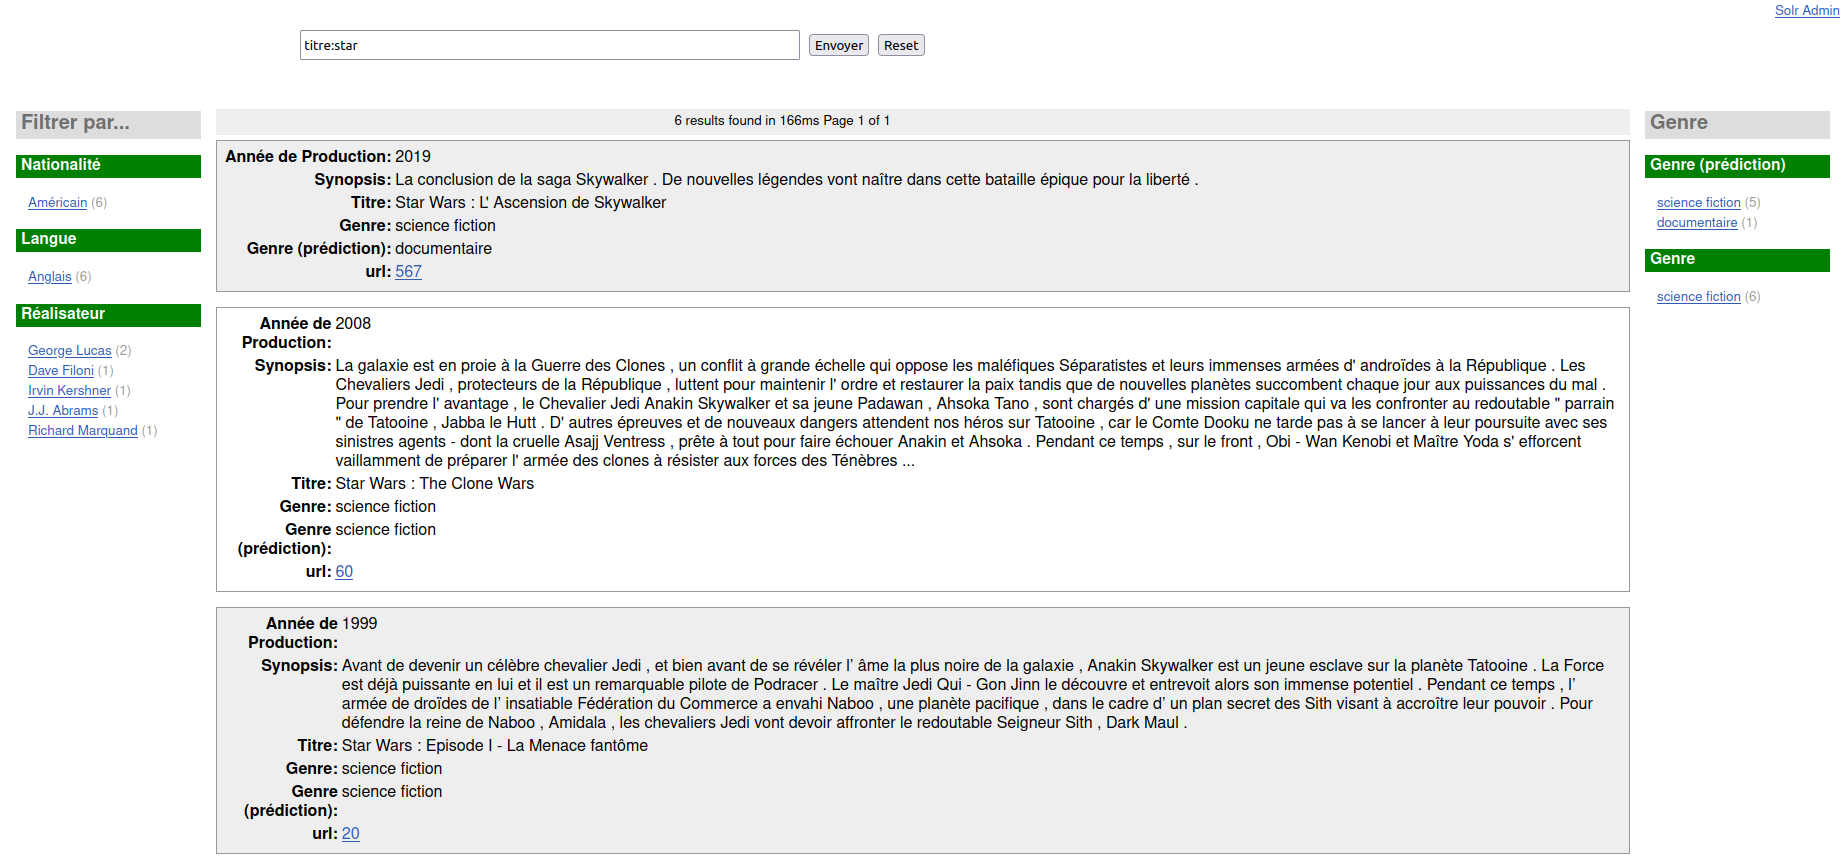
\includegraphics[scale=.25]{img/solr.png}
    \caption{Interface web Solr pour une requête sur le mot \textit{star}}
    \label{solr}
\end{figure}

